\documentclass{article}

\usepackage[italian]{babel}
\usepackage[utf8]{inputenc}
\usepackage{amsmath}
\usepackage{graphicx}
\usepackage{siunitx}
\usepackage[colorlinks=true, allcolors=black]{hyperref}
\usepackage[a4paper]{geometry}
\usepackage{float}
\graphicspath{ {./} }

\title{Prova Finale (Progetto di Reti Logiche)}
\author{Jonathan Sciarrabba (Codice Persona: 10675342 - Matricola: 933553)}
\date{a.a. 2021-2022}

\begin{document}

\maketitle
\tableofcontents
\clearpage


\section{Introduzione}
\subsection{Obiettivo del progetto}
Realizzare un componente descritto in VHDL che data una sequenza di parole, ciascuna di 8 bit, applichi ad essa il codice convoluzionale $1/2$. L'algoritmo consiste nel far corrispondere a ciascun bit letto in ingresso 2 bit in uscita.

\subsection{Specifiche}
Il modulo da realizzare riceve in ingresso una sequenza $U$ di parole, ognuna di 8 bit, e restituisce in uscita una sequenza di parole $Z$, alla sequenza $U$ viene applicato il codice convoluzionale $1/2$ perciò la lunghezza di $Z$ sarà di $2*U$.\\Il codice da applicare al flusso $U$ segue il seguente diagramma di macchina a stati finiti:\\

\begin{figure}[h]
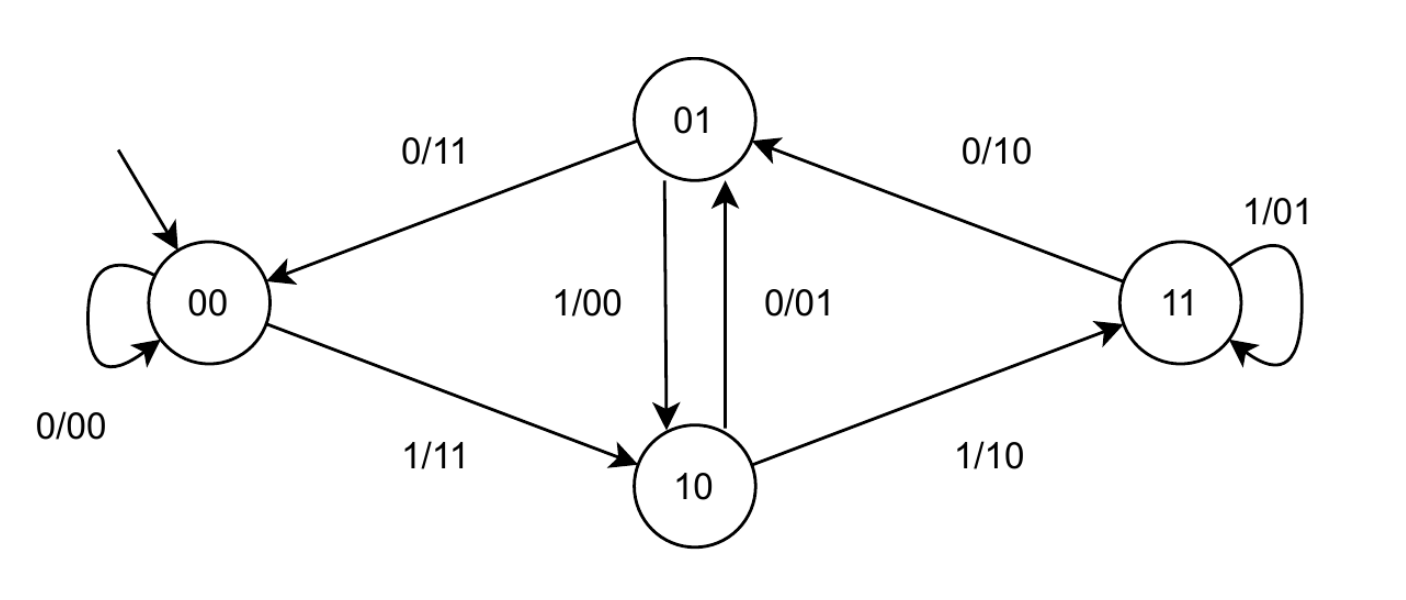
\includegraphics[scale=0.39]{fsm_conv.PNG}
\centering
\caption{Rappresentazione della macchina a stati che realizza il codice convoluzionale}
\centering
\end{figure}
Un esempio di funzionamento con byte in ingresso: $11010110$, si noti che la serializzazione avviene da sinistra verso destra perciò $T_0 = 1$, $T_1 = 1$, $T_2 = 0$, ecc.\\
In questo esempio $U$ corrisponde appunto alla sequenza $11010110$ che verrà codificata nel seguente modo:

\begin{table}[h]
    \centering
    \begin{tabular}{|c|c|c|c|c|c|c|c|c|}
        \hline
         & $T_0$ & $T_1$ & $T_2$ & $T_3$ & $T_4$ & $T_5$ & $T_6$ & $T_7$\\
        \hline 
        $U$ & $1$ & $1$ & $0$ & $1$ & $0$ & $1$ & $1$ & $0$\\
        \hline
        $Z$ & $11$ & $10$ & $10$ & $00$ & $01$ & $00$ & $10$ & $10$\\
        \hline
    \end{tabular}
    \caption{Esempio di codifca}
\end{table}

La sequenza $Z$ in uscita sarà dunque $1110100001001010$ che corrisponde ai 2 byte:
\begin{itemize}
    \item $11101000$
    \item $01001010$
\end{itemize}
 che andranno scritti in memoria.\\
 È presente inoltre un vincolo sul periodo di clock, il componente deve funzionare con un periodo di clock di almeno \SI{100}{\nano\second}.

\subsection{Descrizione memoria}
La memoria da cui il componente descritto legge e scrive è istanziata all'interno del TestBench, il suo funzionamento segue le linee guida della User Guide di VIVADO.\\
I dati all'interno della memoria sono indirizzabili al byte e sono contenuti secondo questo schema:

\begin{table}[h]
    \centering
    \begin{tabular}{ccc}
        
        \cline{1-1}
        \multicolumn{1}{|c|}{\rule[-6.5mm]{0mm}{15mm}Numero di parole da codificare} & $\leftarrow$ & Indirizzo $0$\\
        
        \cline{1-1}
        \multicolumn{1}{|c|}{ \rule[-6.5mm]{0mm}{15mm}Prima parola di $U$} & $\leftarrow$ & Indirizzo $1$\\
        
        \cline{1-1}
        \multicolumn{1}{|c|}{ \rule[-6.5mm]{0mm}{15mm}Seconda parola di $U$} & $\leftarrow$ & Indirizzo $2$\\
        
        \cline{1-1}
        \multicolumn{1}{|c|}{ \rule[-6.5mm]{0mm}{15mm}...} &  & \\
        
        \cline{1-1}
        \multicolumn{1}{|c|}{ \rule[-6.5mm]{0mm}{15mm}Prima parola di $Z$} & $\leftarrow$ & Indirizzo $1000$\\
        
        \cline{1-1}
        \multicolumn{1}{|c|}{ \rule[-6.5mm]{0mm}{15mm}Seconda parola di $Z$} & $\leftarrow$ & Indirizzo $1001$\\
        
        \cline{1-1}
        
    \end{tabular}
    \caption{Rappresentazione schematica della memoria}
\end{table}

\subsection{Interfaccia del componente}
Il componente da descrivere ha una interfaccia così definita:
\begin{verbatim}
entity project_reti_logiche is
    port (
        i_clk : in std_logic;
        i_rst : in std_logic;
        i_start : in std_logic;
        i_data : in std_logic_vector(7 downto 0);
        o_address : out std_logic_vector(15 downto 0);
        o_done : out std_logic;
        o_en : out std_logic;
        o_we : out std_logic;
        o_data : out std_logic_vector (7 downto 0)
    );
end project_reti_logiche;
\end{verbatim}
Nello specifico:
\begin{itemize}
    \item \verb|i_clk|: segnale di \verb|CLOCK| generato dal TestBench
    \item \verb|i_rst|: segnale di \verb|RESET| che inizializza il componente pronto a ricevere il segnale di \verb|START|
    \item \verb|i_start|: segnale di \verb|START| che dà inizio alla codifica 
    \item \verb|i_data|: segnale (vettore) in ingresso che rappresenta il byte letto dalla memoria
    \item \verb|o_address|: segnale (vettore) che manda l'indirizzo alla memoria
    \item \verb|o_done|: segnale di \verb|DONE| che il componente invia al TestBench quando termina la codifica e scrittura di tutte le parole
    \item \verb|o_en|: segnale di \verb|ENABLE| che abilita l'accesso alla memoria sia in lettura che in scrittura
    \item \verb|o_we|: segnale di \verb|WRITE ENABLE| che abilita la scrittura in memoria
    \item \verb|o_data|: segnale (vettore) di uscita che rappresenta il byte da scrivere in memoria
\end{itemize}


\section{Architettura}

\subsection{Macchina a stati sincrona}
Nel modulo realizzato la parte che si occupa di gestire i segnali di input e output rispetto al TestBench si comporta come una macchina a stati finiti che esegue i suoi cambi di stato sul fronte di salita del \verb|CLOCK|.\\Di seguito uno schematico per comprendere meglio il suo funzionamento:

\begin{figure}[H]
\centerline{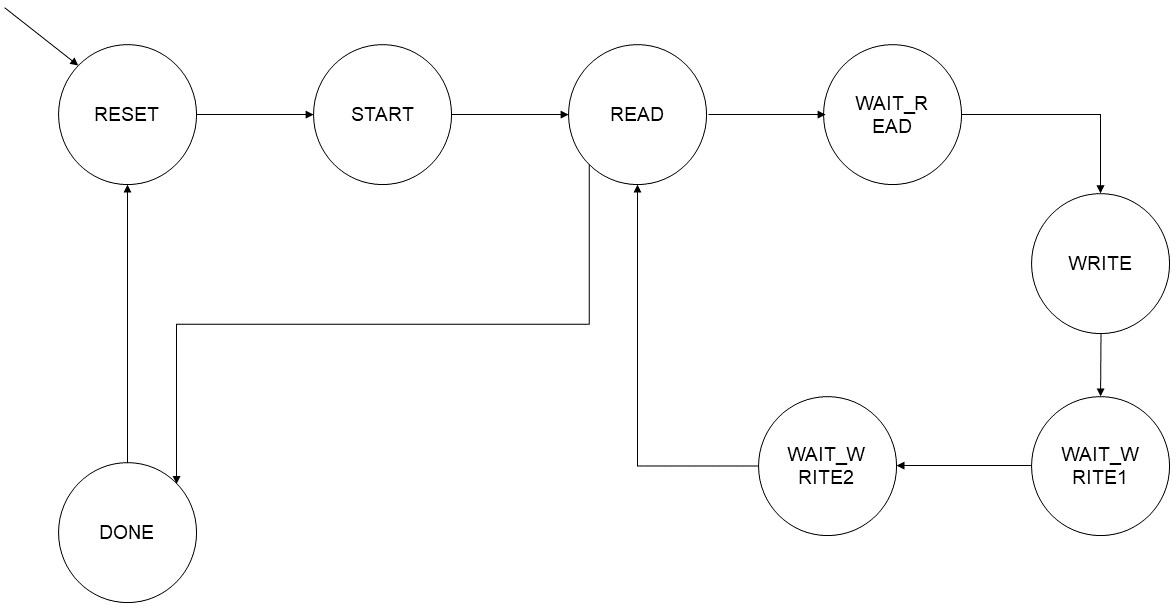
\includegraphics[scale=0.5]{fsm_sincrona.jpg}}
\centering
\caption{Schematico FSM gestione input/output}
\centering
\end{figure}

\begin{itemize}
    \item RESET - stato iniziale, pronto a ricevere il segnale di \verb|START|;
    \item START - stato transitorio per consentire l'accesso corretto alla memoria;
    \item READ - stato che assegna gli indirizzi da leggere alla memoria;
    \item WAIT\_READ - stato che attende la disponibilità del dato in output dalla memoria;
    \item WRITE - stato che esegue il calcolo del codice convoluzionale $1/2$;
    \item WAIT\_WRITE1 - stato di attesa per la scrittura del primo byte;
    \item WAIT\_WRITE2 - stato di attesa per la scrittura del secondo byte;
    \item DONE - stato di terminazione dell'elaborazione, invia il segnale di \verb|DONE|.
\end{itemize}

\subsection{Macchina a stati asincrona}
Il calcolo del codice convoluzionale vero e proprio viene eseguito da una FSM asincrona scritta in una \textit{procedure} richiamata ogni qualvolta si ha un nuovo byte da elaborare che ritorna alla macchina a stati sincrona una sequenza (vettore) di 16 bit che corrispondono ai 2 byte da dover scrivere in memoria.
Il componente riproduce esattamente la FSM presentata in precedenza (vedi Figura 1).\\
Ecco un esempio di codifica effettuata dal modulo:
\\
\begin{figure}[h]
\centerline{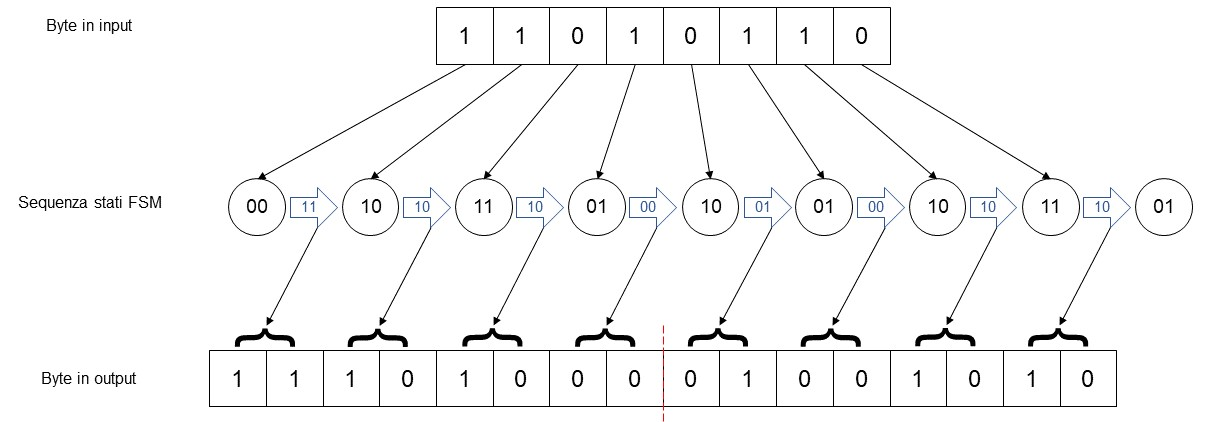
\includegraphics[scale=0.5]{seq_stati_es.jpg}}
\centering
\caption{Esempio di codifica}
\centering
\end{figure}

\clearpage
\section{Risultati Sperimentali}
Sono stati effettuati diversi test per verificare il corretto funzionamento del componente.\\
Nello specifico sono stati effettuati test che andassero a verificare il comportamento desiderato anche nei cosiddetti \textit{corner case}.

\subsection{Testbench memoria vuota}
\textbf{Sequenza di parole da leggere di lunghezza 0 byte:}\\
L'obiettivo del test è quello di verificare il corretto funzionamento del modulo nel caso in cui la sequenza di parole da codificare sia di lunghezza minima (valore $00000000$ all'indirizzo $0$ della memoria).

\begin{figure}[H]
\centerline{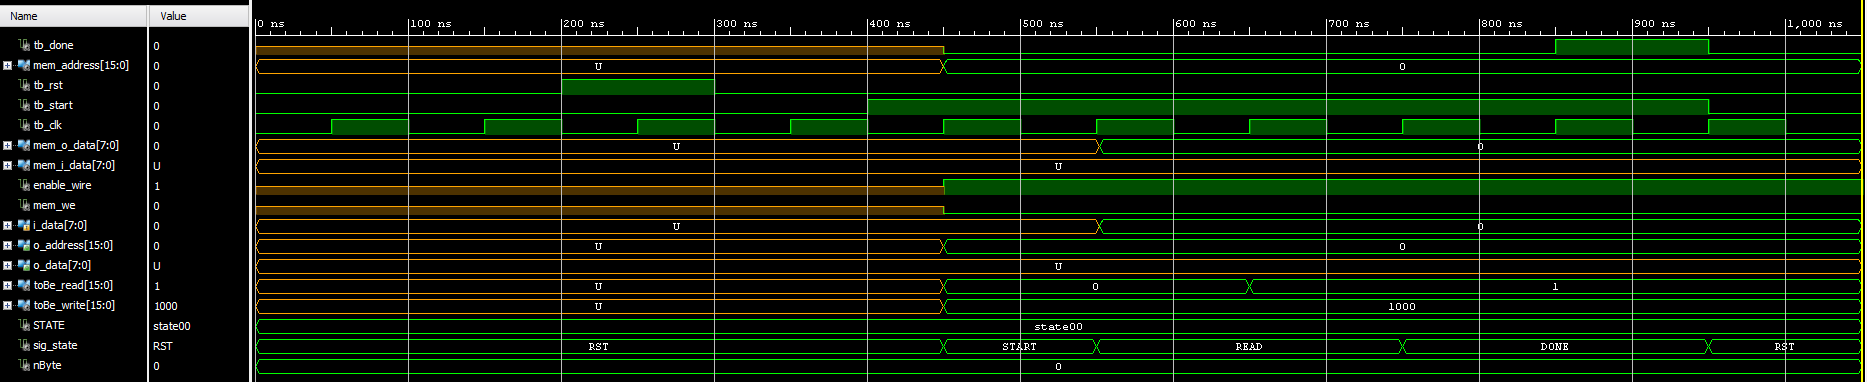
\includegraphics[scale=0.35]{tb_seq_min.PNG}}
\centering
\caption{Forme d'onda del TestBench con sequenza di lunghezza minima}
\centering
\end{figure}

\subsection{Testbench memoria piena}
\textbf{Sequenza di parole da leggere di lunghezza 255 byte:}\\
L'obiettivo del test è quello di verificare il corretto funzionamento del modulo nel caso in cui la sequenza di parole da codificare sia di lunghezza massima (valore $11111111$ all'indirizzo $0$ della memoria).

\begin{figure}[H]
\centerline{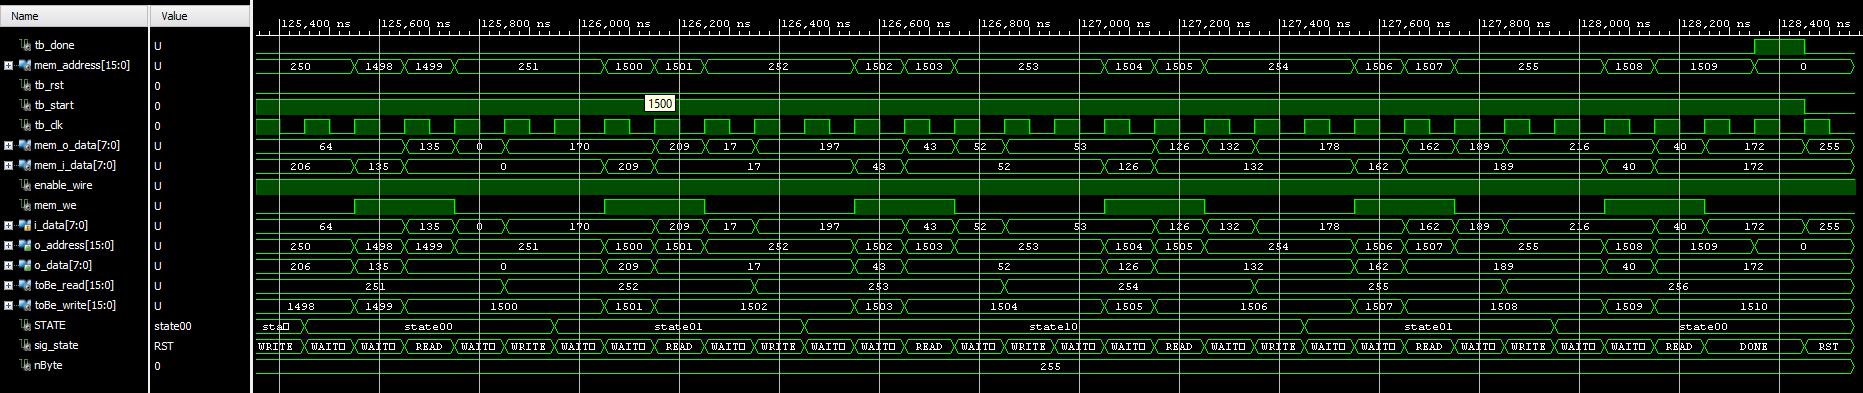
\includegraphics[scale=0.35]{tb_seq_max.PNG}}
\centering
\caption{Forme d'onda del TestBench con sequenza di lunghezza massima (solo parte finale)}
\centering
\end{figure}

\subsection{Testbench codifiche sequenziali}
\textbf{Segnali di} \verb|START| \textbf{multipli:}\\
L'obiettivo del test è quello di verificare il corretto funzionamento del modulo nel caso in cui al termine dell'elaborazione venga dato un nuovo segnale di \verb|START| con conseguente cambio di contenuto in memoria.

\begin{figure}[H]
\centerline{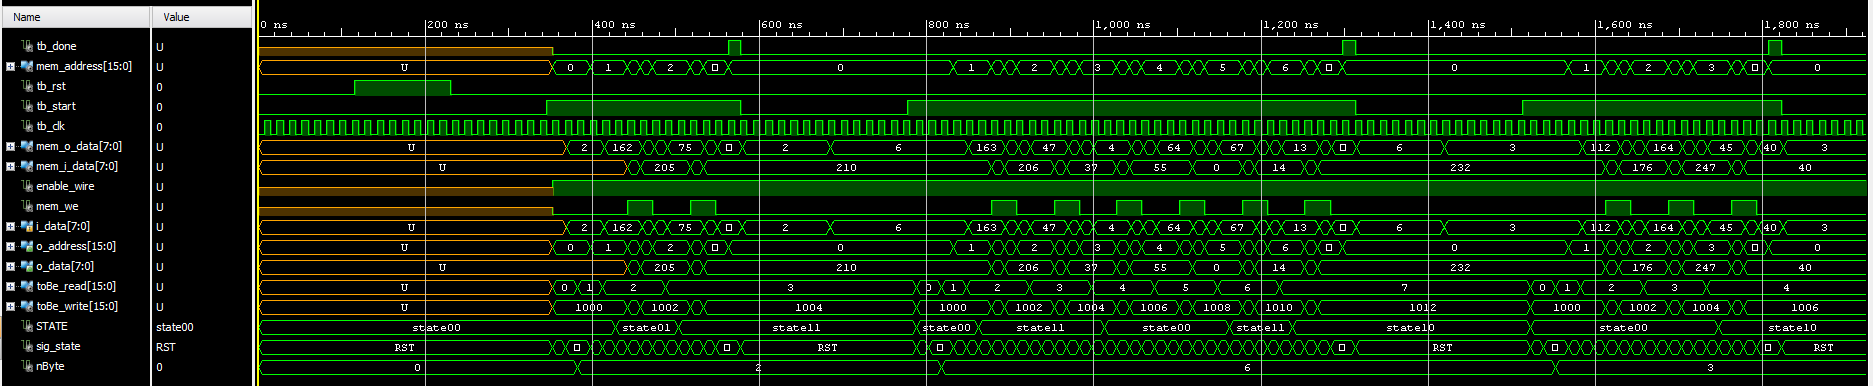
\includegraphics[scale=0.35]{tb_start_multipli.PNG}}
\centering
\caption{Forme d'onda del TestBench con multipli segnali di START}
\centering
\end{figure}

\subsection{Testbench reset multipli}
\textbf{Segnali di} \verb|RESET| \textbf{multipli:}\\
L'obiettivo del test è quello di verificare il corretto funzionamento del modulo nel caso in cui vengano dati segnali di \verb|RESET| (sincroni) casualmente durante l'elaborazione.

\begin{figure}[H]
\centerline{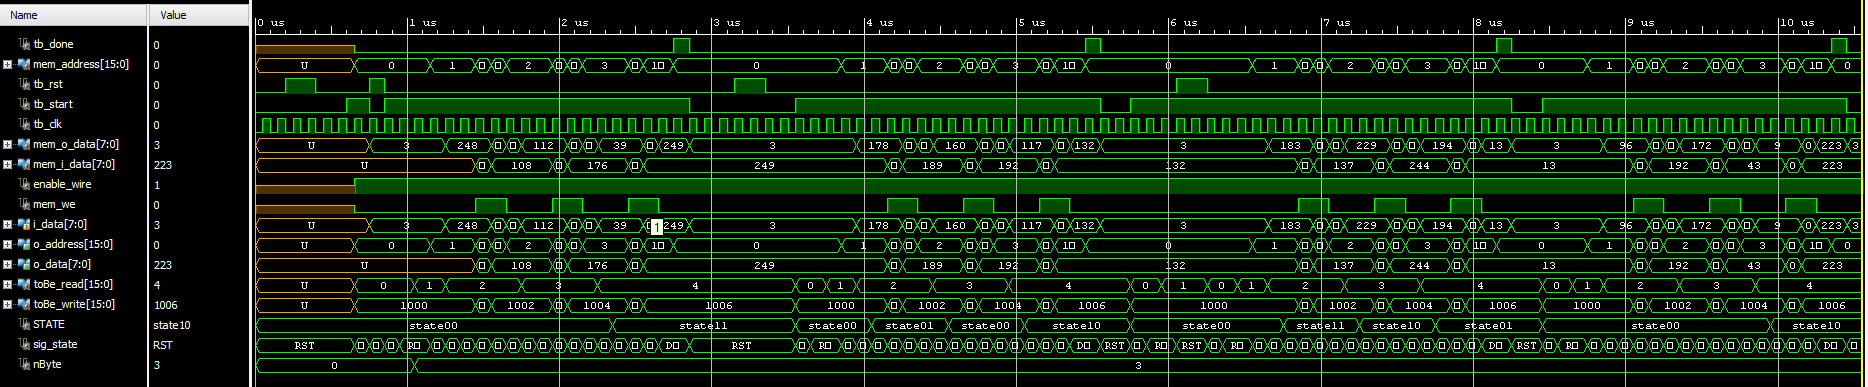
\includegraphics[scale=0.35]{tb_reset_multipli.PNG}}
\centering
\caption{Forme d'onda del TestBench con multipli segnali di RESET}
\centering
\end{figure}

\subsection{Testbench con valori randomici}
\textbf{Test con valori randomici per maggior copertura:}\\
L'obiettivo del test è quello di coprire il maggior numero di scenari possibili, verificando quindi più possibili percorsi di esecuzione. Sono stati quindi eseguiti numerosi test con valori casuali in memoria. 


\section{Conclusione}
Il componente descritto ha concluso con successo tutti i test effettuati in modalità \textit{Behavioral}, \textit{Post-Synthesis Functional} e \textit{Post-Synthesis Timing}.\\
Di seguito sono presentati i tempi di esecuzione nei casi limite:
\begin{itemize}
    \item[-] Caso ottimo: \SI{1,4}{\micro\second}
    \item[-] Caso pessimo: \SI{128,6}{\micro\second}
\end{itemize}
Il caso ottimo corrisponde al caso in cui la sequenza da codificare sia di $0$ parole, Il caso peggiore invece corrisponde al caso in cui la sequenza da codificare sia di $255$ parole.

\subsection{Report timings}
Dopo la sintesi è possibile verificare i timings del modulo e si può notare come il ciclo di clock possa scendere fino a circa \SI{5}{\nano\second} senza causare malfunzionamenti, siccome il \textit{Worst Negative Slack} è di circa \SI{95}{\nano\second} su \SI{100}{\nano\second} di periodo di clock disponibile.

\begin{figure}[H]
\centerline{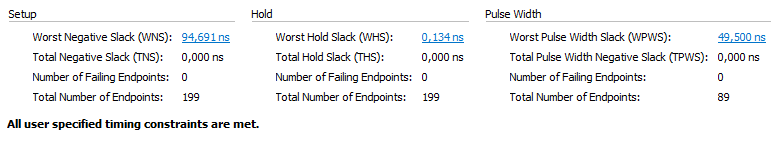
\includegraphics[height=3cm]{timing.PNG}}
\centering
\caption{Report timings all'interno di VIVADO}
\centering
\end{figure}

\subsection{Report utilization}
Sempre dopo la sintesi è possibile verificare l'utilizzo di \textit{LUT, Flip-Flop e Latch}. Quest'ultimi non sono presenti nel componente sintetizzato poiché darebbero origine a un circuito non più puramente combinatorio.

\begin{figure}[H]
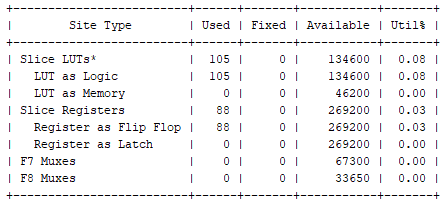
\includegraphics{utilization.PNG}
\centering
\caption{Report utilization all'interno di VIVADO}
\centering
\end{figure}

\end{document}